\documentclass[../main.tex]{subfiles}

\begin{document}

\subsection{Utformning}

Efter att läst på och bekantat mig med skatter, ritades ett strukturdiagram\\

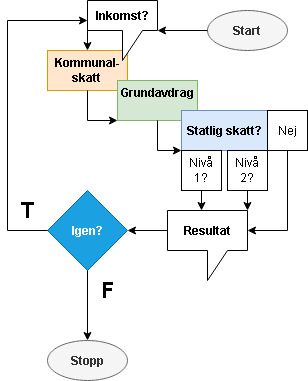
\includegraphics[width=11cm, height=10cm]{Projekt/Inkomstskatt/figs/strukturdiagram01.jpg}
\\
Sedan underlättar vi konstruktionens detaljerade nivåer, genom att bryta ned diagrammet i sektioner,

\begin{tcolorbox}[colback=gray!5!white,colframe=black!75!black]

\begin{enumerate}

    \item \textbf{Indata}. Här tilldelas programmet användarens årliga bruttoinkomst.
    
    \item \textbf{Sekvens}. Beräknar kommunalskatt, grundavdraget och statlig skatt. 
    
    \item \textbf{Selektion}. Här beskrivs valet av skiktgränsen till den statliga skatten. Tillhör den beskattningsbara inkomsten nedre eller övre skiktgränsen.
    
    \item \textbf{Utdata}. Presentationen av resultaten till användaren.
    
    \item \textbf{Iteration.} Låter användaren mata in ett nytt värde.
    
\end{enumerate}

\end{tcolorbox}

\newpage

\end{document}